%% Geometry of circles %%
% Question 3
\question Find the equation of the tangent to each circle at the point 
specified:
\begin{parts}
	%%%%%%%%%%%%%%%%%%%%%%%%%%%%%
	% part a
	%%%%%%%%%%%%%%%%%%%%%%%%%%%%%
	\part circle 
		\(
			x^{2} + y^{2} - 2x - 4y - 20 = 0
		\), 
		point $(4,-2)$;
	\begin{solution}
		BE note: $(1 + 4 - r^{2} = -20)$
		\[
			(x-1)^{2} + (y-2)^{2} = 5^{2}
		\]
		\[
			\therefore
			\text{centre} \; 
			(1, 2)
			,\; \text{radius} = 
			5
		\]
		Calculate gradient of normal
		\newline
		For: $(1, 2) \leftrightarrow (4, -2)$, using: 
		\[
			\frac{y - y_{1}}{y_{2} - y_{1}}
			=
			\frac{x - x_{1}}{x_{2} - x_{1}}
			\quad
			\&
			\quad
			m_{1} m_{2} = -1
		\]
		\[
			\frac{y - 2}{-2 - 2}
			=
			\frac{x - 1}{4 - 1}
		\]
		\[
			y =	-\frac{4}{3}x + \frac{4}{3} + 2
		\]
		\[
			y =	-\frac{4}{3}x + \frac{10}{3}
		\]
		\[
			m_{2} = \frac{3}{4}
		\]
		Sub in $y = mx + c$
		\[
			\rightarrow
			(-2) = \frac{3}{4}(4) + c
		\]
		\[
			c = -5
		\]
		\qSolMath{
			y = \frac{3}{4}x - 5
		}{}
		\underline{Diagram:}
		\begin{center}
			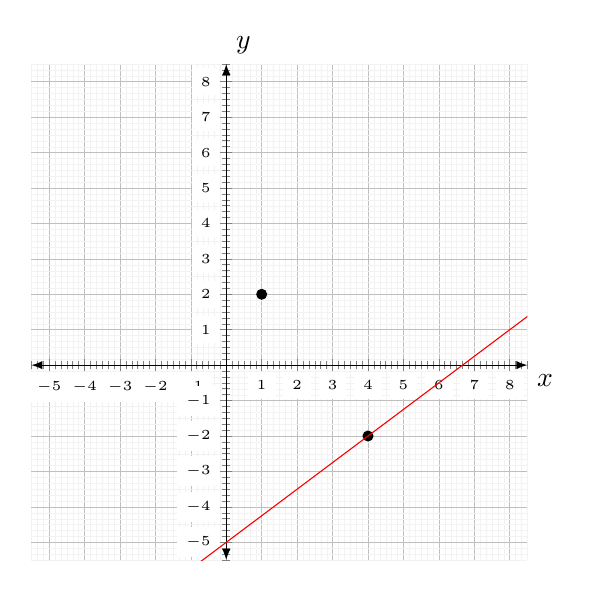
\begin{tikzpicture}
				\begin{axis}[
						width=0.65\textwidth,
						height=0.65\textwidth,
						xtick distance=1,
						ytick distance=1,
						xmin=-5.0,xmax=8,
						ymin=-5.0,ymax=8,
						xlabel = $x$,
						ylabel = $y$,
						grid=both,
						grid style={line width=.1pt, draw=gray!10},
						major grid style={line width=.2pt,draw=gray!50},
						axis lines=middle,
						minor tick num=5,
						enlargelimits={abs=0.5},
						axis line style={latex-latex},
						ticklabel style={font=\tiny,fill=white},
						xlabel style={at={(ticklabel* cs:1)},anchor=north west},
						ylabel style={at={(ticklabel* cs:1)},anchor=south west},
					]
					\fill (axis cs: 1, 2) circle[radius=2pt];
					\draw (axis cs: 1, 2) circle[radius=500];
					\fill (axis cs: 4, -2) circle[radius=2pt];
					
					\addplot [
						domain=-5:10, 
						samples=100, 
						color=red,
					]
					{ (3*x)/4 - 5};
				\end{axis}
			\end{tikzpicture}
		\end{center}
			
	\end{solution}

	%%%%%%%%%%%%%%%%%%%%%%%%%%%%%
	% part b
	%%%%%%%%%%%%%%%%%%%%%%%%%%%%%
	\part circle 
		\(
			x^{2} + y^{2} +4x +2y - 20 = 0
		\), 
		point $(1,3)$;
	\begin{solution}
		BE note: $(4 + 1 - r^{2} = -20)$
		\[
			(x+2)^{2} + (y+1)^{2} = 5^{2}
		\]
		\[
			\therefore
			\text{centre} \; 
			(-2, -1)
			,\; \text{radius} = 
			5
		\]
		Calculate gradient of normal
		\newline
		For: $(-2, -1) \leftrightarrow (1, 3)$, using: 
		\[
			\frac{y - y_{1}}{y_{2} - y_{1}}
			=
			\frac{x - x_{1}}{x_{2} - x_{1}}
			\quad
			\&
			\quad
			m_{1} m_{2} = -1
		\]
		\[
			\frac{y +1}{3 +1}
			=
			\frac{x +2}{1 +2}
		\]
		\[
			y + 1 =	\frac{4}{3}x + \frac{8}{3}
		\]
		\[
			y =	\frac{4}{3}x + \frac{5}{3}
		\]
		\[
			m_{2} = -\frac{3}{4}
		\]
		Sub in $y = mx + c$
		\[
			\rightarrow
			(3) = -\frac{3}{4}(1) + c
		\]
		\[
			c = \frac{15}{4}
		\]
		\qSolMath{
			y = -\frac{3}{4}x + \frac{15}{4}
		}{}
		\underline{Diagram:}
		\begin{center}
			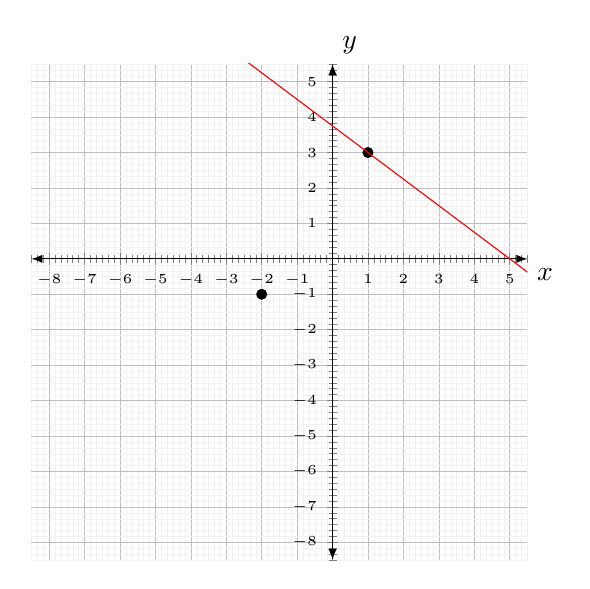
\begin{tikzpicture}
				\begin{axis}[
						width=0.65\textwidth,
						height=0.65\textwidth,
						xtick distance=1,
						ytick distance=1,
						xmin=-8.0,xmax=5,
						ymin=-8.0,ymax=5,
						xlabel = $x$,
						ylabel = $y$,
						grid=both,
						grid style={line width=.1pt, draw=gray!10},
						major grid style={line width=.2pt,draw=gray!50},
						axis lines=middle,
						minor tick num=5,
						enlargelimits={abs=0.5},
						axis line style={latex-latex},
						ticklabel style={font=\tiny},
						xlabel style={at={(ticklabel* cs:1)},anchor=north west},
						ylabel style={at={(ticklabel* cs:1)},anchor=south west},
					]
					\fill (axis cs: -2, -1) circle[radius=2pt];
					\draw (axis cs: -2, -1) circle[radius=500];
					\fill (axis cs: 1, 3) circle[radius=2pt];
					
					\addplot [
						domain=-8:6, 
						samples=100, 
						color=red,
					]
					{ -(3*x)/4 + (15/4)};
				\end{axis}
			\end{tikzpicture}
		\end{center}
			
	\end{solution}

	%%%%%%%%%%%%%%%%%%%%%%%%%%%%%
	% part c
	%%%%%%%%%%%%%%%%%%%%%%%%%%%%%
	\part circle 
		\(
			x^{2} + y^{2} -6x +4y - 87 = 0
		\), 
		point $(-3,-10)$;
	\begin{solution}
		BE note: $(9 + 4 - r^{2} = -87)$ 
		\vspace{-0.1\baselineskip}
		\[
			(x-3)^{2} + (y+2)^{2} = 10^{2}
		\]
		\[
			\therefore
			\text{centre} \; 
			(3, -2)
			,\; \text{radius} = 
			5
		\]
		Calculate gradient of normal
		\newline
		For: $(3, -2) \leftrightarrow (-3, -10)$, using: 
		\[
			\frac{y - y_{1}}{y_{2} - y_{1}}
			=
			\frac{x - x_{1}}{x_{2} - x_{1}}
			\quad
			\&
			\quad
			m_{1} m_{2} = -1
		\]
		\[
			\frac{y +10}{(-2) - (-10)}
			=
			\frac{x -(-3)}{3 - (-3)}
		\]
		\[
			y + 10 = \frac{8}{6} \left( x + 3 \right)
		\]
		\[
			y =	\frac{4}{3}x -6
		\]
		\[
			m_{2} = -\frac{3}{4}
		\]
		Sub in $y = mx + c$
		\[
			\rightarrow
			(-10) = \left( -\frac{3}{4} \right) (-3) + c
		\]
		\[
			c 
			= -10 - \frac{9}{4}
			= -\frac{49}{4}
		\]
		\qSolMath{
			y = -\frac{3}{4}x - \frac{49}{4}
		}{}
		\underline{Diagram:}
		\begin{center}
			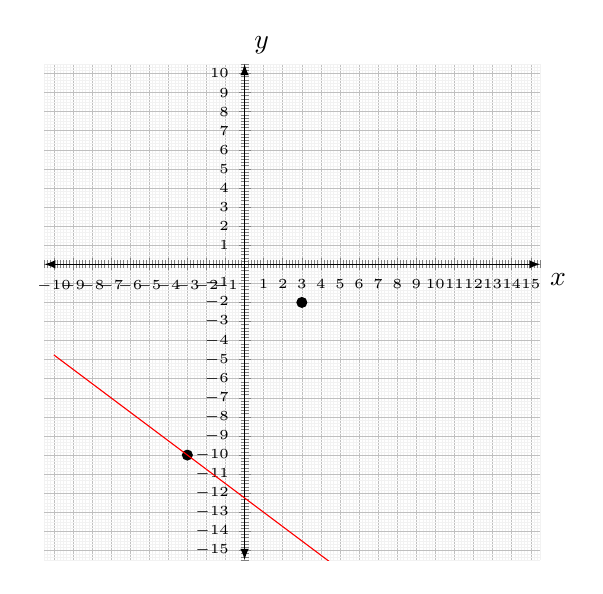
\begin{tikzpicture}
				\begin{axis}[
						width=0.65\textwidth,
						height=0.65\textwidth,
						xtick distance=1,
						ytick distance=1,
						xmin=-10.0,xmax=15,
						ymin=-15.0,ymax=10,
						xlabel = $x$,
						ylabel = $y$,
						grid=both,
						grid style={line width=.1pt, draw=gray!10},
						major grid style={line width=.2pt,draw=gray!50},
						axis lines=middle,
						minor tick num=5,
						enlargelimits={abs=0.5},
						axis line style={latex-latex},
						ticklabel style={font=\tiny},
						xlabel style={at={(ticklabel* cs:1)},anchor=north west},
						ylabel style={at={(ticklabel* cs:1)},anchor=south west},
					]
					\fill (axis cs: 3, -2) circle[radius=2pt];
					\draw (axis cs: 3, -2) circle[radius=100];
					\fill (axis cs: -3, -10) circle[radius=2pt];
					
					\addplot [
						domain=-10:11, 
						samples=100, 
						color=red,
					]
					{ -(3*x)/4 - (49/4)};
				\end{axis}
			\end{tikzpicture}
		\end{center}
			
	\end{solution}

	%%%%%%%%%%%%%%%%%%%%%%%%%%%%%
	% part d
	%%%%%%%%%%%%%%%%%%%%%%%%%%%%%
	\part circle 
		\(
			x^{2} + y^{2} +18x - 88 = 0
		\), 
		point $(3, 5)$;
	\begin{solution}
		BE note: $(81 - r^{2} = -88 \rightarrow r^{2} = 169)$
		\[
			(x+9)^{2} + (y+0)^{2} = 13^{2}
		\]
		\[
			\therefore
			\text{centre} \; 
			(-9, 0)
			,\; \text{radius} = 
			13
		\]
		Calculate gradient of normal
		\newline
		For: $(-9, 0) \leftrightarrow (3, 5)$, using: 
		\[
			\frac{y - y_{1}}{y_{2} - y_{1}}
			=
			\frac{x - x_{1}}{x_{2} - x_{1}}
			\quad
			\&
			\quad
			m_{1} m_{2} = -1
		\]
		\[
			\frac{y -0}{5 - 0}
			=
			\frac{x +9}{3 + 9}
		\]
		\[
			y = \frac{5}{12} \left( x + 9 \right)
		\]
		\[
			y =	\frac{5}{12}x + \frac{45}{12}
		\]
		\[
			m_{2} = -\frac{12}{5}
		\]
		Sub in $y = mx + c$
		\[
			\rightarrow
			(5) = \left( -\frac{12}{5} \right) (3) + c
		\]
		\[
			c 
			= 5 + \frac{36}{5}
			= \frac{61}{5}
		\]
		\qSolMath{
			y = -\frac{12}{5}x + \frac{61}{5}
		}{}
		\underline{Diagram:}
		\begin{center}
			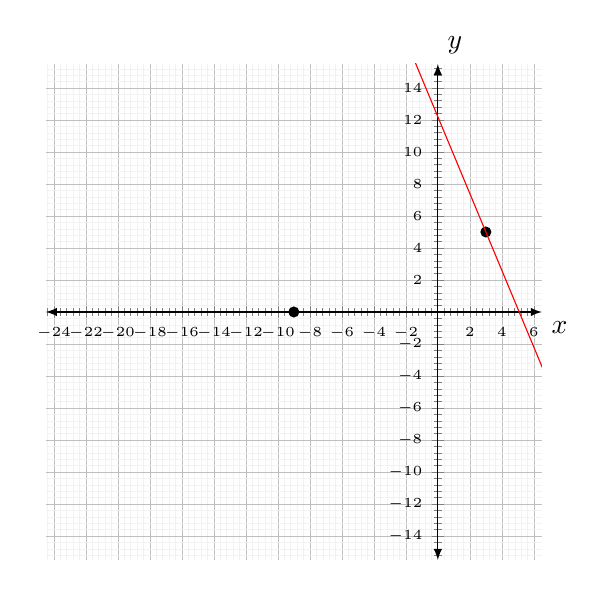
\begin{tikzpicture}
				\begin{axis}[
						width=0.65\textwidth,
						height=0.65\textwidth,
						xtick distance=2,
						ytick distance=2,
						xmin=-24.0,xmax=6,
						ymin=-15.0,ymax=15,
						xlabel = $x$,
						ylabel = $y$,
						grid=both,
						grid style={line width=.1pt, draw=gray!10},
						major grid style={line width=.1pt,draw=gray!50},
						axis lines=middle,
						minor tick num=4,
						enlargelimits={abs=0.5},
						axis line style={latex-latex},
						ticklabel style={font=\tiny},
						xlabel style={at={(ticklabel* cs:1)},anchor=north west},
						ylabel style={at={(ticklabel* cs:1)},anchor=south west},
					]
					\fill (axis cs: -9, 0) circle[radius=2pt];
					\draw (axis cs: -9, 0) circle[radius=130];
					\fill (axis cs: 3, 5) circle[radius=2pt];
					
					\addplot [
						domain=-10:11, 
						samples=100, 
						color=red,
					]
					{ -(12*x)/5 + (61/5)};
				\end{axis}
			\end{tikzpicture}
		\end{center}
			
	\end{solution}

	%%%%%%%%%%%%%%%%%%%%%%%%%%%%%
	% part e
	%%%%%%%%%%%%%%%%%%%%%%%%%%%%%
	\part circle 
		\(
			x^{2} + y^{2} -6y - 160 = 0
		\), 
		point $(12, 8)$;
	\begin{solution}
		BE note: $(9 - r^{2} = -160)$
		\[
			(x+0)^{2} + (y-3)^{2} = 13^{2}
		\]
		\[
			\therefore
			\text{centre} \; 
			(0, 3)
			,\; \text{radius} = 
			13
		\]
		Calculate gradient of normal
		\newline
		For: $(0, 3) \leftrightarrow (12, 8)$, using: 
		\[
			\frac{y - y_{1}}{y_{2} - y_{1}}
			=
			\frac{x - x_{1}}{x_{2} - x_{1}}
			\quad
			\&
			\quad
			m_{1} m_{2} = -1
		\]
		\[
			\frac{y -3}{8 - 3}
			=
			\frac{x -0}{12 - 0}
		\]
		\[
			y - 3 = \frac{5}{12}x
		\]
		\[
			y =	\frac{5}{12}x + 3
		\]
		\[
			m_{2} = -\frac{12}{5}
		\]
		Sub in $y = mx + c$
		\[
			\rightarrow
			(8) = \left( -\frac{12}{5} \right) (12) + c
		\]
		\[
			c 
			= 8 + \frac{144}{5}
			= \frac{184}{5}
		\]
		\qSolMath{
			y = -\frac{12}{5}x + \frac{184}{5}
		}{}
		\underline{Diagram:}
		\begin{center}
			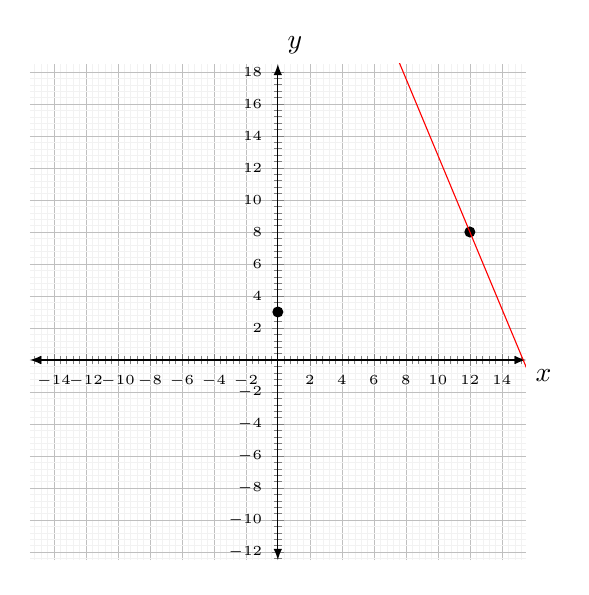
\begin{tikzpicture}
				\begin{axis}[
						width=0.65\textwidth,
						height=0.65\textwidth,
						xtick distance=2,
						ytick distance=2,
						xmin=-15.0,xmax=15,
						ymin=-12.0,ymax=18,
						xlabel = $x$,
						ylabel = $y$,
						grid=both,
						grid style={line width=.1pt, draw=gray!10},
						major grid style={line width=.1pt,draw=gray!50},
						axis lines=middle,
						minor tick num=4,
						enlargelimits={abs=0.5},
						axis line style={latex-latex},
						ticklabel style={font=\tiny},
						xlabel style={at={(ticklabel* cs:1)},anchor=north west},
						ylabel style={at={(ticklabel* cs:1)},anchor=south west},
					]
					\fill (axis cs: 0, 3) circle[radius=2pt];
					\draw (axis cs: 0, 3) circle[radius=130];
					\fill (axis cs: 12, 8) circle[radius=2pt];
					
					\addplot [
						domain=0:18, 
						samples=100, 
						color=red,
					]
					{ -(12*x)/5 + (184/5)};
				\end{axis}
			\end{tikzpicture}
		\end{center}
			
	\end{solution}

\end{parts}

\appenddata{questionSolutions}{
{
\begin{parts}
	% a
	\part {
		$y = \frac{3}{4}x - 5$
		$\;$
		or
		$\;$
		$4y = 3x - 20$
	}
	% b
	\part {
		$y = -\frac{3}{4}x + \frac{15}{4}$
		$\;$
		or
		$\;$
		$4y + 3x = 15$
	}
	% c
	\part {
		$y = -\frac{3}{4}x - \frac{49}{4}$
		$\;$
		or
		$\;$
		$4y + 3x + 49 = 0$
	}
	% d
	\part {
		$y = -\frac{12}{5}x + \frac{61}{5}$
		$\;$
		or
		$\;$
		$5y + 12x = 61$
	}
	% e
	\part {
		$y = -\frac{12}{5}x + \frac{184}{5}$
		$\;$
		or
		$\;$
		$5y + 12x = 184$
	}
\end{parts}
}
}